%-*- coding: utf-8 -*-
\label{chap:dimred}

\paragraph{Notions :} sélection de variables ; extraction de variables ;
 analyse en composantes principales ; analyse en composantes principales probabiliste.
\paragraph{Objectifs pédagogiques :} 
\begin{itemize}      
  \setlength{\itemsep}{3pt}
\item Expliquer l'intérêt de réduire la dimension d'un jeu de données ;
\item Faire la différence entre la sélection de variables et l'extraction de variables ;
% \item Mettre en \oe{}uvre des méthodes de sélection de variable par filtrage ;
\item Projeter des données sur un espace de plus petite dimension ;%par factorisation de matrice ; 
\item Mettre en \oe{}uvre des méthodes d'extraction de variables.
\end{itemize}

\section{Des séries statistiques aux jeux de données}
Nous avons jusqu'à présent travaillé sur des séries statistiques contenant une
seule variable. Cependant, dans la majorité des problèmes de science des
données, nous disposons de plusieurs variables pour décrire chaque individu.

L'objet de nos études, à savoir le jeu de données, n'est donc plus un
échantillon $(x_1, x_2, \dots, x_n)$ d'une variable aléatoire réelle $X$, mais
d'un \textit{vecteur} aléatoire à valeurs dans un espace $\XX$. Nous
considèrerons en général que $\XX = \RR^p$ et que notre jeu de données peut
être décrit par une matrice $X \in \RRnp$.  C'est par exemple la
matrice de taille $31 \times 8$ des entrées du tableau~\ref{tab:meteo_data}.

Cela suppose que nous disposions d'une représentation $p$-dimensionnelle
pertinente de nos données. Si celle-ci est assez évidente pour des données
comme celles du tableau~\ref{tab:meteo_data}, ce n'est pas toujours le cas. En
particulier, les variables qualitatives (comme la colonne « âge » du
tableau~\ref{tab:remboursement_data}) doivent être représentées par un (ou
plusieurs) nombres réels. 

Nous supposons dans ce cours que nos données sont présentées sous forme
vectorielle ; on parle parfois de données \textbf{structurées}. Ce n'est pas le
cas de nombreux types de données telles que du texte, des images, du son, des
séquences d'ADN, ou des molécules chimiques. La question de la représentation
de ces données dites non-structurées dépasse le cadre de ce cours mais est très
importante.

\section{Notations}
Nous essaierons à partir de maintenant de nous en tenir aux notations suivantes
:
\begin{itemize}
\item Les lettres minuscules ($x$) représentent un scalaire ;
\item les lettres minuscules surmontées d'une flèche ($\xx$) représentent un
  vecteur ;
\item les lettres majuscules ($X$) représentent une matrice, un événement ou
  une variable aléatoire ;
\item les lettres calligraphiées ($\XX$) représentent un ensemble ou un espace ;
\item les {\it indices} correspondent à une variable tandis que les {\it
    exposants} correspondent à une observation : $x^i_j$ est la $j$-ème
  variable de la $i$-ème observation, et correspond à l'entrée $X_{ij}$ de la
  matrice $X$ ;
\item $n$ est un nombre d'observations et $p$ un nombre de variables.
\end{itemize}

\section{Motivation $\bullet$}
Le but de la réduction de dimension est de transformer une représentation
$X \in \RRnp$ des données en une représentation
$X^* \in \RR^{n \times m}$ où $m \ll p$. Les raisons de cette démarche sont
multiples.

\paragraph{Visualiser les données.} Ce n'est pas tâche aisée avec un nombre
très grand de variables. Comment visualiser $n$ points en plus de 2 ou 3
dimensions ? Limiter les variables à un faible nombre de dimensions permet de
visualiser les données plus facilement, quitte à perdre un peu d'information
lors de la transformation.

\paragraph{Réduire les coûts algorithmiques du traitement des données.} D'un
point de vue purement computationnel, réduire la dimension des données permet
de réduire d'une part l'espace qu'elles prennent en mémoire et d'autre part les
temps de calcul. De plus, si certaines variables sont inutiles, ou redondantes,
il n'est pas nécessaire de les obtenir pour de nouvelles observations : cela
permet de réduire le coût d'acquisition des données.

\paragraph{Améliorer la qualité du traitement des données.} Les algorithmes
d'apprentissage supervisé ou de clustering sont généralement plus performants
sur un faible nombre de variables. En effet, si certaines des variables
ne sont pas pertinentes, elles risquent de biaiser les modèles appris.\\
De plus, les raisonnements développés en faible dimension pour construire un
algorithme d'apprentissage supervisé ne s'appliquent pas nécessairement en
haute dimension. C'est un phénomène connu sous le nom de \textbf{fléau de la
  dimension}, ou \textit{curse of dimensionality} en anglais. \\
En effet, en haute dimension, les individus ont tendance à tous être éloignés
les uns des autres. Pour comprendre cette assertion, plaçons-nous en dimension
$p$ et considérons l'hypersphère $\Scal(\xx, R)$ de rayon $R \in \RR_+^*$
centrée sur une observation $\xx$, ainsi que l'hypercube $\Ccal(\xx, R)$
circonscrit à cette hypersphère. Le volume de $\Scal(\xx)$ vaut
$\frac{R^p \pi^{p/2}}{\Gamma(1+p/2)}$, tandis que celui de $\Ccal(\xx, R)$,
dont le côté a pour longueur $2R$, vaut $2^p R^p$. Ainsi
\begin{equation*}
  \lim_{p \rightarrow \infty} \frac{\text{Vol}(\Scal(\xx, R))}{
    \text{Vol}(\Ccal(\xx, R))} = 0.
\end{equation*}
Cela signifie que la probabilité qu'une observation située dans $\Ccal(\xx, R)$
appartienne à $\Scal(\xx, R)$, qui vaut $\frac{\pi}4 \approx 0.79$ lorsque
$p=2$ et $\frac{\pi}6 \approx 0.52$ lorsque $p=3$, devient très faible quand
$p$ est grand : les données ont tendance à être éloignées les unes des autres.

% Cela implique que les algorithmes développés en utilisant une notion de
% similarité ou distance entre individus ne fonctionnent pas nécessairement en
% grande dimension. Ainsi, réduire la dimension des données peut être nécessaire
% à la construction de bons modèles d'apprentissage.

Deux possibilités s'offrent à nous pour réduire la dimension de nos données :
\begin{itemize}
\item la \textbf{sélection de variables}, qui consiste à \textit{éliminer} un nombre
  $(p-m)$ de variables de nos données ;
\item l'\textbf{extraction de variables}, qui consiste à {\it créer} $m$
  nouvelles variables à partir des $p$ variables dont nous disposons
  initialement.
\end{itemize}



\section{Sélection de variables $\bullet$} 

La sélection de variables consiste à éliminer des variables peu informatives.

Dans le cas non-supervisé, il s'agit par exemple d'éliminer des variables:
\begin{itemize}
\item dont la variance est très faible : leur valeur étant à peu près la même
  pour chaque individu, elles n'apportent aucune information permettant de
  distinguer deux individus ;
\item qui sont corrélées à une autre variable : elles apportent alors la même
  information et sont redondantes.
\end{itemize}

Dans le cas supervisé, il s'agit aussi d'éliminer des variables qui ne sont pas
pertinentes par rapport à la tâche de prédiction. On peut par exemple:
\begin{itemize}
\item éliminer, par exemple à l'aide d'un test statistique ou une mesure de corrélation,
  les variables indépendantes de l'étiquette à prédire. Remarquez néanmoins que
  deux variables chacune indépendante de l'étiquette peuvent être très
  informatives quand on les considère simultanément. Considérez par exemple,
  pour $\XX = \zo^2$, un problème de classification binaire dans lequel
  l'étiquette $y$ est donnée par $y = x_1 \oplus x_2$ : les deux variables
  prises ensemble déterminent parfaitement $y,$ mais chacune d'entre elles
  prise individuellement est décorrélée de $y$ ;
\item chercher à éliminer des variables qui n'améliorent pas la performance
  d'un algorithme précis.
\end{itemize}
Nous reviendrons sur la
sélection de variables supervisée quand nous parlerons du lasso
(section~\ref{sec:lasso}).


%La suite de ce chapitre détaille des exemples de ces deux approches.

\section{Analyse en composantes principales $\bullet$}
\label{sec:pca}
La méthode la plus classique pour réduire la dimension d'un jeu de données par
extraction de variables est l'\textbf{analyse en composantes principales}, ou
{\it ACP}. On parle aussi souvent de {\it PCA}, de son nom anglais {\it
  Principal Component Analysis}.

\subsection{Maximisation de la variance $\bullet$}
\label{sec:variance_maximization}
L'idée est de représenter les données selon leurs axes de plus grande
variation, de sorte à pouvoir continuer à distinguer les observations les unes
des autres dans leur nouvelle représentation
(cf. figure~\ref{fig:data_variance}).  Ainsi, une ACP de la matrice
$X \in \RRnp$ est une transformation linéaire orthogonale qui permet d'exprimer
$X$ dans une nouvelle base orthonormée, de sorte à maximiser la variance de la
projection de $X$ sur les axes de cette nouvelle base. De plus, on ordonne ces
axes, appelés \textbf{composantes principales}, abrégées en {PC} pour {\it
  Principal Components}, par variance décroissante.
Plus précisément, étant donné $m \leq p$, on appelle $m$ composantes
principales de $X \in \RRnp$ une liste $(\ww_1, \ww_2, \ldots, \ww_m)$ de
vecteurs $\ww_j$ de $\RR^p$, vérifiant, pour tout $j = 1, \dots, m$ :
\begin{equation}
  \left\lbrace
    \begin{split}
      & \ww_j \in \argmax_{\ww \in \RR^p} \text{var}(X \ww) \\
      & \ltwonorm{\ww_j} = 1 \\
      & \langle \ww_j, \ww_k \rangle = 0  \text{ pour tout } k < j
    \end{split}
  \right.
  \label{eq:pc_def}
\end{equation}
  


\begin{figure}[h!]
  \centering
  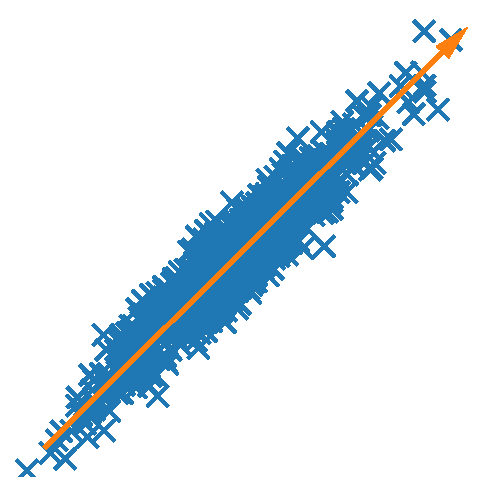
\includegraphics[width=0.3\textwidth]{figures/dimred/data_variance}
  \caption{La variance des données en deux dimensions est maximale selon l'axe
    indiqué par la flèche.}
  \label{fig:data_variance}
\end{figure}


\subsection{Standardisation}
Dans la suite de cette section, nous supposons que les variables ont été
\textbf{standardisées} de sorte à toutes avoir une moyenne de 0 et une variance
de 1, pour éviter que les variables qui prennent de grandes valeurs aient plus
d'importance que celles qui prennent de faibles valeurs. C'est un pré-requis de
l'application de l'ACP.  Cette standardisation s'effectue par :
\begin{equation}
  \label{eq:standardization}
  x^i_j \leftarrow \frac{x^i_j - \overline{x_j}}{\sqrt{\frac1n 
      \sum_{l=1}^n (x^l_j - \overline{x_j})^2}},
\end{equation}
où $\overline{x_j} = \frac1n \sum_{l=1}^n x^l_j.$ On dira alors que $X$ est
\textbf{centrée}, i.e. chacune de ses colonnes a pour moyenne 0, et \textbf{réduite}, i.e. chacune de ses colonnes a pour variance 1.

\begin{exemple}
  Considérons la matrice de données 
  \[
    X = \begin{bmatrix} 1.0 & 20.0 \\
      2.0 & 10.0 \\
      3.0 & 50.0 \\
      4.0 & 30.0 \\
      5.0 & 40.0 \\
    \end{bmatrix}.
  \]
  La variance de la première colonne vaut $2.0$ tandis que celle de la deuxième
  colonne vaut $200.0$. Peut-on pour autant en conclure que la deuxième
  variable « varie » plus que la première, alors que les valeurs qu'elle prend
  sont simplement proportionnelles à celles prises par la première ?

  La version standardisée de $X$ est
  \[
    \begin{bmatrix} -1.414 & -0.707 \\
      -0.707 & -1.414 \\
      0.0 & 1.414 \\
      0.707 & 0.0 \\
      1.414 & 0.707 
    \end{bmatrix}.
  \]
\end{exemple}


\subsection{Décomposition spectrale de la covariance $\bullet$}
\paragraph{Matrice de covariance} La matrice de covariance empirique d'une matrice de
données $X \in \RRnp$ est une matrice $\Sigma \in \RRpp$ telle que
$\Sigma_{jk} = \text{cov}\left(\xx_j, \xx_k \right)$ pour tout
$j, k = 1, \ldots, p$. Ici $\xx_j \in \RR^n$ représente la série statistique
composée des $n$ observations de la $j$-ème variable. Ainsi, si les données
sont centrées-réduites,
\[
  \Sigma_{jk} = \frac1n \sum_{i=1}^n (x_j^i - \overline{x_j})  (x_k^i - \overline{x_k}) = \frac1n \sum_{i=1}^n x_j^i x_k^i
   = \frac1n \langle \xx_j, \xx_k \rangle
 \]
 et $\Sigma = \frac1n X^\top X$ est une matrice symétrique avec $\frac1n$ sur la diagonale (car $\Sigma_{jj} = \text{var}(\xx_j) = 1$).

\paragraph{Proposition} 
Soit $X \in \RRnp$ une matrice centrée et 
$\Sigma = \frac1n X^\top X$ sa matrice de covariance empirique. Les composantes principales de $X$ sont les
vecteurs propres de $\Sigma$, ordonnés par valeurs propres décroissantes.

\paragraph{Preuve  $\bullet\bullet$}
\begin{itemize}
\item Considérons un vecteur $\ww \in \RR^p$. 
La moyenne de $X \ww$ vaut $0$ car les variables $(\xx_1, \dots, \xx_p)$ sont
elles-mêmes de moyenne nulle ($X$ étant centrée).
La variance de $X \ww$ vaut donc 
\begin{equation*}
  \text{var}(X \ww) = \frac1n \sum_{i=1}^n \left( \sum_{j=1}^p x_j^i w_j \right)^2 = \ww^\top \Sigma \ww.
\end{equation*}    
\item Appelons maintenant $\ww_1 \in \RR^p$ la première composante principale de $X$.
Le vecteur $\ww_1$ est de norme $1$ et tel que la variance de $X \ww_1$ est maximale :
\begin{equation}
  \label{eq:pc1}
  \ww_1 \in \argmax_{\ww \in \RR^p} \left( \ww^\top \Sigma \ww \right)  \text{\qquad avec } \ltwonorm{\ww_1}^2=1.
\end{equation}
Il s'agit d'un problème d'optimisation quadratique sous contrainte d'égalité,
que l'on peut résoudre (cf section 2.2.1 du poly d'Optimisation) en
introduisant le multiplicateur de Lagrange $\alpha_1 > 0$ et en écrivant le
lagrangien
\begin{equation*}
  L(\alpha_1, \ww) = \ww^\top \Sigma \ww - \alpha_1 
  \left( \ltwonorm{\ww}^2 - 1 \right).
\end{equation*}
%Par dualité forte, % $\min_{\ww \in \RR^p} w^\top \Sigma w = \max_{\alpha_1}
    % \inf_{\ww \in \RR^p} L(\alpha_1, \ww).$
Le maximum de $\ww^\top \Sigma \ww$ sous la contrainte $\ltwonorm{\ww_1}^2=1$ est
égal à $\min_{\alpha_1} \sup_{\ww \in \RR^p} L(\alpha_1, \ww).$ Le supremum du
lagrangien est atteint en un point où son gradient s'annule, c'est-à-dire qui
vérifie
\begin{equation*}
  2 \Sigma \ww - 2 \alpha_1 \ww = 0.
\end{equation*}
Ainsi, $\Sigma \ww_1 = \alpha_1 \ww_1$ et $(\alpha_1, \ww_1)$ forment un couple
(valeur propre, vecteur propre) de $\Sigma$.

Parmi tous les vecteurs propres de $\Sigma$, $\ww_1$ est celui qui maximise la
variance $\ww_1^\top \Sigma \ww_1 = \alpha_1 \ltwonorm{\ww_1} = \alpha_1.$
Ainsi, $\alpha_1$ est la plus grande valeur propre de $\Sigma$ (rappelons que
$\Sigma$ étant définie par $X^\top X$ est semi-définie positive et que toutes
ses valeurs propres sont positives).

\item La deuxième composante principale de $X$ vérifie
\begin{equation}
  \label{eq:pc2}
  \ww_2 = \argmax_{\ww \in \RR^p} \left( \ww^\top \Sigma \ww \right) \text{ \qquad avec } \ltwonorm{\ww_2}^2=1
  \text{ et } \ww_2^\top\ww_1=0.
\end{equation}

Nous introduisons donc maintenant deux multiplicateurs de Lagrange
$\alpha_2 > 0$ et $\beta_2 > 0$ et obtenons le lagrangien
\begin{equation*}
  L(\alpha_2, \beta_2, \ww) = \ww^\top \Sigma \ww - \alpha_2 
  \left(\ltwonorm{\ww}^2 - 1 \right)
  - \beta_2 \ww^\top\ww_1.
\end{equation*}
Comme précédemment, son supremum en $\ww$ est atteint en un point où son
gradient s'annule :
\begin{equation*}
  2 \Sigma \ww_2 - 2 \alpha_2 \ww_2 - \beta_2 \ww_1 = 0.
\end{equation*}
En multipliant à gauche par $\ww_1^\top$, on obtient
\begin{equation*}
  2 \ww_1^\top \Sigma \ww_2 - 2 \alpha_2 \ww_1^\top \ww_2 - 
  \beta_2 \ww_1^\top \ww_1 = 0.
\end{equation*}
Comme $\ww_1^\top \Sigma \ww_2 = 0$ puisque les $\xx_j$ sont centrées, et que
$\ww_1^\top \ww_2 = 0$ et $\ww_1^\top \ww_1 = 1$ par définition
(équation~\eqref{eq:pc2}), on en conclut que $\beta_2=0.$ En remplaçant dans
l'équation précédente, comme pour $\ww_1$, on obtient
$2 \Sigma \ww_2 - 2 \alpha_1 \ww_2 = 0$.  Ainsi $(\alpha_2, \ww_2)$ forment un
couple (valeur propre, vecteur propre) de $\Sigma,$ distinct de
$(\alpha_1, \ww_1),$ et $\alpha_2$ est maximale : il s'agit donc nécessairement
de la deuxième valeur propre de $\Sigma$.
    
\item Le raisonnement se poursuit de la même manière pour les composantes principales
  suivantes.
\end{itemize}
\hfill $\square$

  
\paragraph{Preuve alternative  $\bullet\bullet$} Alternativement, on peut prouver ce théorème
en observant que $\Sigma$, étant définie positive, est
diagonalisable par un changement de base orthonormée :
$\Sigma = Q^\top \Lambda Q$, où $\Lambda \in \RRpp$ est une
matrice diagonale dont les valeurs diagonales $\lambda_1,\dots,\lambda_p$ sont les valeurs propres de
$\Sigma$.  Ainsi,
\begin{equation*}
  \ww_1^\top \Sigma \ww_1 = \ww_1^\top Q^\top \Lambda Q \ww_1 = 
  \left(Q \ww_1 \right)^\top \Lambda \left(Q \ww_1 \right).
\end{equation*}
Si l'on pose $\vv = Q \ww_1$, il s'agit donc pour maximiser
$\ww_1^\top \Sigma \ww_1$ de trouver $\vv$ de norme 1 ($Q$ étant orthonormée et
$\ww_1$ de norme 1) qui maximise
\[\sum_{j=1}^p v_j^2 \lambda_j.\]  

Pour tout $j=1, \dots, p$, on a $\lambda_j \geq 0$ (car $\Sigma$ est définie
positive) et $0 \leq v_j^2 \leq 1$ car $\ltwonorm{\vv} = 1$. Ainsi, 
\[\sum_{j=1}^p v_j^2 \lambda_j \leq 
\left(\max_{j=1, \dots, p} \lambda_j \right)\sum_{j=1}^p
v_j^2 \leq \max_{j=1, \dots, p} \lambda_j,\]
et ce maximum est atteint quand $v_j=1$ et $v_k=0 \text{ pour tout } k \neq j$. On
retrouve ainsi que $\ww_1$ est le vecteur propre correspondant à la plus grande
valeur propre de $\Sigma$, et ainsi de suite. \hfill $\square$


\subsection{Décomposition en valeurs singulières $\bullet\bullet$}
\paragraph{Définition/Proposition} Toute matrice $X \in \RRnp$ peut être
décomposée sous la forme $X = U D V^\top,$ avec $U \in \RR^{n \times n}$ et
$V \in \RRpp$ orthogonales et $D \in \RRnp$ une matrice diagonale positive
(c'est-à-dire que ses coefficients diagonaux $D_{ii}$ pour
$i=1, \dots, \min(n, p)$ sont positifs ou nuls et les coefficients hors
diagonale sont nuls).

Cette décomposition est appelée \textbf{décomposition en valeurs singulières},
ou \textit{SVD} pour \textit{Singular Value Decomposition}, et les
coefficients diagonaux $D_{ii}$ sont les \textbf{valeurs singulières} de $X$,
c'est-à-dire les racines des valeurs propres de $X^\top X$. 

\paragraph{Preuve} La matrice $X^\top X$ étant positive semi-définie, il existe d'après le théorème spectral une matrice orthogonale $V \in \RRpp$ telle que
\begin{equation}
  V^\top \left( X^\top X\right) V =
  \begin{bmatrix}
    \Delta & 0 \\
    0 & 0
  \end{bmatrix}
  \label{eq:diag_xtx}
\end{equation}
avec $\Delta \in \RR^{r \times r}$ diagonale, de coefficients strictement positifs, de même rang $r \leq \min(n, p)$ que $X.$ 

En décomposant $V$ en deux blocs : $V =
\begin{bmatrix}
  V_1 & V_2 \\
\end{bmatrix}$ avec $V_1 \in \RR^{p \times r}$ et $V_2 \in \RR^{p \times (p-r)}$, on peut réécrire l'équation~\eqref{eq:diag_xtx} comme
\begin{equation*}
  \begin{bmatrix}
    V_1^\top X^\top X V_1 & V_1^\top X^\top X V_2 \\
    V_2^\top X^\top X V_1 & V_2^\top X^\top X V_2
  \end{bmatrix} =  
  \begin{bmatrix}
    V_1^\top \\
    V_2^\top
  \end{bmatrix}  \left( X^\top X\right) 
  \begin{bmatrix}
    V_1 & V_2
  \end{bmatrix} =
  \begin{bmatrix}
    \Delta & 0 \\
    0 & 0
  \end{bmatrix}
\end{equation*}
et identifier $V_1^\top X^\top X V_1 = \Delta$.
% et $V_2^\top X^\top X V_2 = 0$, ce qui implique $X V_2 = 0$ (la trace de $V_2^\top X^\top X V_2$ étant la somme des carrés des entrées de $X V_2$).

Posons maintenant $U_1 = (X V_1) \Delta^{-1/2} \in \RR^{n \times r}.$
$U_1^\top U_1 = \Delta^{-1/2} (X V_1)^\top  (X V_1) \Delta^{-1/2} = I_r$ et on peut étendre les colonnes orthonormées de $U_1$ par $U_2 \in \RR^{n \times (n-r)}$ de sorte à former une base orthonormée de $\RRnn$ et obtenir $U =
\begin{bmatrix}
  U_1 U_2
\end{bmatrix}$ orthogonale.

Enfin, posons
\begin{equation*}
  D =
  \begin{bmatrix}
    \Delta^{1/2} & 0 \\
    0 & 0 \\
  \end{bmatrix}
\end{equation*}
avec $D \in \RR^{n \times p}$ -- autrement dit, on ajoute $(p-r) \geq 0$ colonnes de zéros
et $(n-r) \geq 0$ lignes de zéros à $\Delta^{1/2}$.

On a maintenant
\begin{equation*}
  U D V^\top =
  \begin{bmatrix}
    U_1 & U_2
  \end{bmatrix}   \begin{bmatrix}
    \Delta^{1/2} & 0 \\
    0 & 0 \\
  \end{bmatrix}
  \begin{bmatrix}
    V_1^\top \\
    V_2^\top
  \end{bmatrix} = U_1 \Delta^{1/2} V_1^\top = (X V_1) \Delta^{-1/2} \Delta^{1/2} V_1^\top = X.
\end{equation*} \hfill $\square$


\paragraph{Relation entre SVD et PCA}
Ainsi, les composantes principales d'une matrice centrée sont ses vecteurs
singuliers à droite (les colonnes de $V$), ordonnés par valeur singulière
décroissante.

\paragraph{Preuve}
Factorisons $X$ sous la forme $U D V^\top$ avec $U \in \RRnn$ et
$V \in \RRpp$ orthogonales, et $D \in \RRnp$ diagonale (c'est-à-dire que les
coefficients $D_{ij}$ pour $i \neq j$ sont nuls) dont les coefficients
diagonaux sont les valeurs singulières de $X$. Alors
\begin{equation*}
 n \Sigma = X^\top X = V D U^\top U D V^\top = V D^2 V^\top
\end{equation*}
et les valeurs singulières de $X$ (les coefficients diagonaux de $D$) sont les racines carrées
des valeurs propres de $n \Sigma$, tandis que les vecteurs singuliers à droite de
$X$ (les colonnes de $V$) sont les vecteurs propres de $n \Sigma$. \hfill $\square$
  
% En pratique, les implémentations de la décomposition en valeurs singulières (ou
% SVD) sont numériquement plus stables que celles de décomposition spectrale, et
% c'est ainsi que l'ACP est implémentée.

\subsection{Choix du nombre de composantes principales $\bullet$}
Réduire la dimension des données par une ACP implique de {\it choisir} un
nombre de composantes principales à conserver. Pour ce faire, on utilise la
\textbf{proportion de variance expliquée} par ces composantes.

La proportion de variance de la matrice de données $X \in \RRnp$ expliquée
par ses $m$ premières composantes est calculée comme :
\begin{equation}
  \label{eq:var_explained}
  \frac{\sum_{j=1}^m \text{var}(X \ww_j)}{\sum_{j=1}^p \text{var}(X \ww_j)} = \frac{\alpha_1 + \alpha_2 + \dots + \alpha_m}{\text{trace}(\Sigma)},
\end{equation}
où $\alpha_1 \geq \alpha_2 \geq \dots \geq \alpha_p$ sont les valeurs propres
de $\Sigma$ par ordre décroissant.
  
Il est classique de s'intéresser à l'évolution, avec le nombre de composantes,
soit de la proportion de variance expliquée par chacune d'entre elles, soit à
cette proportion cumulée. On peut représenter visuellement ces proportions sur
un {\it scree plot} (figure~\ref{fig:scree_plots}), utilisé pour déterminer le
nombre de composantes qui expliquent ensemble un pourcentage de la variance
fixé a priori ($95\%$ sur la figure~\ref{fig:scree_plot_cumul}), ou le nombre
de composantes à partir duquel ajouter une nouvelle composante n'est plus
informatif («~coude~» sur la
figure~\ref{fig:scree_plot}). % Ce graphe peut nous servir
% à déterminer visuellement soit le nombre de composantes principales qui
% expliquent un pourcentage de la variance que l'on s'est initialement fixé
% ($95\%$ sur la figure~\ref{fig:scree_plot}, soit le nombre de composantes
% principales correspondant au « coude » du scree plot cumulatif
% (figure~\ref{fig:scree_plot_cumul}), à partir duquel ajouter une nouvelle
% composante ne semble plus informatif.


\begin{figure}[h]
  \begin{subfigure}[t]{0.43\textwidth}
    \centering
    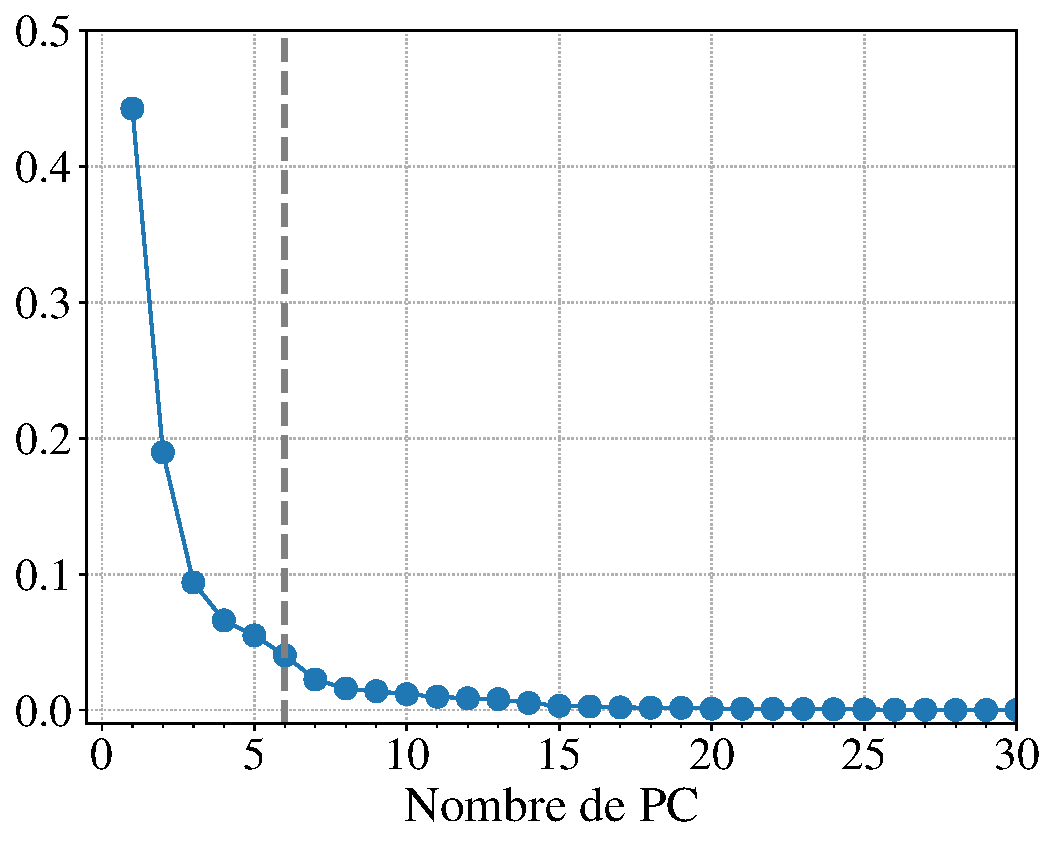
\includegraphics[width=\textwidth]{figures/dimred/scree_plot}
    \caption{Proportion de variance expliquée par chacune des composantes
      principales. À partir de 6 composantes principales, ajouter de nouvelles
      composantes n'est plus vraiment informatif.}
    \label{fig:scree_plot}
  \end{subfigure} \hfill
  \begin{subfigure}[t]{0.43\textwidth}
    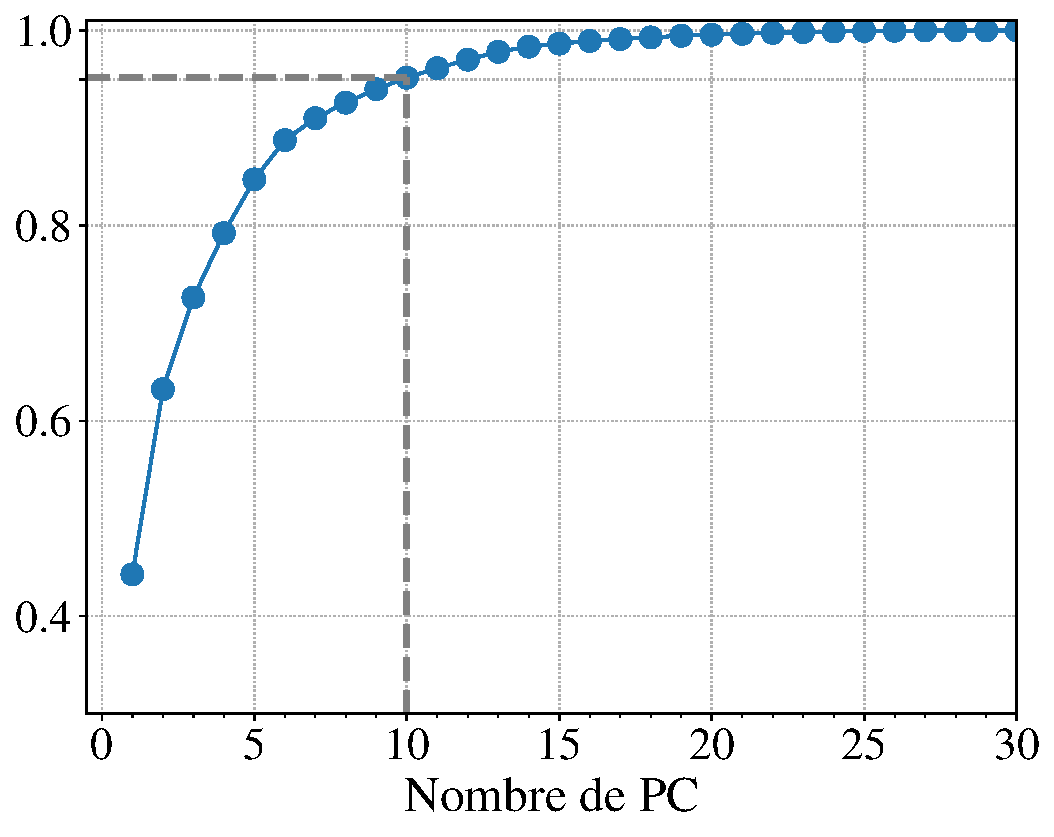
\includegraphics[width=\textwidth]{figures/dimred/scree_plot_cumul}  
    \caption{Proportion cumulée de variance expliquée par chacune des
      composantes principales. Si on se fixe une proportion de variance
      expliquée de $95\%$, on peut se contenter de 10 composantes principales.}
    \label{fig:scree_plot_cumul}
  \end{subfigure}
  \caption{Choix du nombre de composantes principales à l'aide de la variance expliquée.}
  \label{fig:scree_plots}
\end{figure}

\section{Factorisation de la matrice des données $\bullet$}
Soit $W \in \RRpp$ la matrice de toutes les composantes principales de
$X \in \RRnp$. Posons $m< p$ le nombre de composantes principales choisies, et
$\widetilde{W} \in \RR^{p \times m}$ la matrice des $m$ premières composantes
principales de $X$ (autrement dit la concaténation des composantes principales
$\ww_1, \ww_2, \dots, \ww_m$ exprimés comme vecteurs colonnes). La nouvelle
représentation dans $\RR^m$ d'un individu $\xx \in \RR^p$ est donnée par sa
projection sur $(\ww_1, \ww_2, \dots, \ww_m)$ :
\begin{equation}
  \label{eq:reduced_rep_vector}
  \hh = \xx \widetilde{W}.
\end{equation}

On obtient la représentation $m$-dimensionnelle des $n$ individus de $X$ par
\begin{equation}
  \label{eq:reduced_rep}
  \widetilde{H} = X \widetilde{W}.
\end{equation}

La matrice $\widetilde{H} \in \RR^{m \times n}$ peut être interprétée comme une
\textbf{représentation latente} (ou cachée, {\it hidden} en anglais d'où la
notation $H$) des données. C'est cette représentation que l'on a cherché à
découvrir grâce à l'ACP.


\subsection{Erreur de reconstruction $\bullet$}
Si on utilise toutes les composantes, la représentation latente de $X$ est donnée par 
\begin{equation}
  \label{eq:full_rep}
  H = X W; H \in \RRnp.
\end{equation}
Les colonnes de $W$ étant des vecteurs orthonormés (il s'agit de vecteurs
propres de $X^\top X$), on peut multiplier l'équation~\eqref{eq:full_rep} à
droite par $W^\top$ pour obtenir une factorisation de $X$ :
\begin{equation}
  \label{eq:pca_factor}
  X = H W^\top.
\end{equation}

En se restreignant à $m < p$ composantes, la multiplication à droite par
$\widetilde{W}^\top$ de la représentation latente $\widetilde{H}$ est une approximation de
$X$ :
\begin{equation}
  \label{eq:pca_factor_approx}
  Z = \widetilde{H} \widetilde{W}^\top.
\end{equation}
$Z \in \RRnp$ peut être interprétée comme une
\textbf{reconstruction} des données dans $\RR^p$ à partir de leur
représentation latente dans $\RR^m$.

On peut alors calculer l'\textbf{erreur de reconstruction} comme la somme des
carrés des distances entre les individus $\xx^i$ et leur reconstruction $\zz^i$ :
\begin{equation}
  \label{eq:pca_reconstruction_error}
  \text{Err}_m = \sum_{i=1}^n \norm{\xx^i - \zz^i}^2.
\end{equation}

L'erreur de reconstruction vaut 
\[
  \text{Err}_m = \sum_{i=1}^n \; \bignorm{\sum_{j=1}^p H_{ij} \ww_j - \sum_{j=1}^m H_{ij} \ww_j }^2 = 
\sum_{i=1}^n \; \bignorm{\sum_{j=m+1}^p H_{ij} \ww_j }^2 = \sum_{i=1}^n \sum_{j=m+1}^p H_{ij}^2,
\]
cette dernière égalité venant de ce que les vecteurs $\ww_j$ sont orthogonaux
et de norme 1.  Ainsi, l'erreur de reconstruction est la somme des carrés des
coefficients des dimensions qui n'ont pas été prises en compte.

Comme $H = X W$, on peut réécrire l'erreur de reconstruction comme 
\[
  \text{Err}_m = \sum_{i=1}^n \sum_{j=m+1}^p \ww_j^\top \xx^i \xx^{i\top}\ww_j
  = \sum_{j=m+1}^p \ww_j \Sigma \ww_j^\top.
\]
Ainsi, maximiser la variance $\sum_{j=1}^m \ww_j \Sigma \ww_j^\top$ est
équivalent à minimiser l'erreur de reconstruction car
$
\sum_{j=1}^p \ww_j \Sigma \ww_j^\top = \text{trace}(\Sigma).
$
C'est une autre justification de l'ACP.

\subsection{Analyse factorielle $\bullet \bullet$}
L'équation \eqref{eq:pca_factor} s'inscrit dans le cadre plus général de
\textbf{l'analyse factorielle}. Il correspond à considérer que les données sont
les réalisations d'un vecteur aléatoire $(X_1, X_2, \dots, X_p)$ obtenues par
% \begin{equation}
%   \label{eq:fa_model}
%   (X_1, X_2, \dots, X_p)^\top = (H_1, H_2, \dots, H_m)^\top W + \epsilon,
% \end{equation}
\begin{equation}
  \label{eq:fa_model}
  (X_1, X_2, \dots, X_p) = W (H_1, H_2, \dots, H_m) + \epsilon,
\end{equation}
où $(H_1, H_2, \dots, H_m)$ est le vecteur aléatoire latent qui génère les
données et $\epsilon$ un bruit gaussien : $\epsilon \sim \Ncal(0, \Psi),$ avec
$\Psi \in \RRpp$.

Supposons maintenant que $(H_1, H_2, \dots, H_m)$ est un vecteur aléatoire
gaussien $m$-dimensionnel, d'espérance $0$ (les variables latentes sont elles
aussi centrées) et de covariance $I_m$ où $I_m$ est la matrice identité de
dimensions $m \times m$. Alors $(X_1, X_2, \dots, X_p)$ est lui-même un vecteur
aléatoire gaussien, d'espérance nulle et de covariance $WW^\top + \Psi$.

Si l'on suppose de plus que $\epsilon$ est un bruit isotropique, autrement dit
que $\Psi = \sigma^2 I_p$, alors 
\[
  (X_1, X_2, \dots, X_p) \sim \Ncal (0, WW^\top + \sigma^2 I_p).
\] 
On peut alors estimer les paramètres $W$ et $\sigma^2$ par maximum de
vraisemblance ; c'est ce qu'on appelle l'\textbf{ACP probabiliste}.

L'ACP que nous venons de voir est un cas limite de l'ACP probabiliste, obtenu
quand la covariance du bruit devient infiniment petite
($\sigma^2 \rightarrow 0$)\footnote{Vous en trouverez la preuve dans l'article
  \textit{Probabilistic principal components analysis}, M.~E. Tipping \&
  C.~M. Bishop,  Journal of the Royal
    Statistical Society Series B, 61:611--622 (1999).}.

On peut plutôt faire la supposition plus générale que $\Psi$ est une matrice
diagonale. Les valeurs de $W$ et $\Psi$ peuvent une fois de plus
être obtenues par maximum de vraisemblance. C'est ce que l'on appelle
\textbf{l'analyse factorielle}.  Dans l'analyse factorielle, les composantes
principales (les colonnes de $W$) ne sont pas nécessairement orthogonales. En
particulier, il est donc possible d'obtenir des composantes dégénérées,
autrement dit des colonnes de $W$ dont toutes les coordonnées sont $0$.

\begin{plusloin}
\item Une variante populaire de l'analyse factorielle est la
  \textbf{factorisation positive de matrice} (ou NMF pour \textit{non-negative
    matrix factorisation}), qui permet lorsque toutes les entrées de $X$ sont
  positives, de chercher à la décomposer sous la forme $H W$ où $H$ et $W$ ont
  elles aussi toutes leurs entrées positives. Cela facilite leur
  interprétation.
\item Il existe de nombreuses approches de réduction de dimension
  non-linéaires, autrement dit qui permettent de construire des composantes qui
  ne sont pas des composantes linéaires des variables initiales. Parmi elles :
  \begin{itemize}
  \item le \textbf{positionnement multidimensionnel}, ou MDS pour {\it
      multidimensional scaling}, qui cherche à préserver la distance entre les
    individus. Dans le cas de la distance euclidienne, on se ramène à l'ACP ;
    mais il est possible d'utiliser d'autres distances, y compris des distances
    non-métriques.
  \item le \textbf{t-SNE} (prononcé « ti-sni »), pour {\it t-Student
      Neighborhood Embedding}, qui cherche à approcher la loi des distances
    entre individus par une loi de Student.
  \item le \textbf{UMAP}, pour {\it Uniform Manifold Approximation and
      Projection} qui suppose les individus uniformément distribués sur une
    variété riemanienne qu'il s'agit d'approcher.
  \end{itemize}
\item Enfin, nous verrons au chapitre~\ref{chap:nonlin} que la dernière couche
  cachée d'un réseau de neurones profond peut être considérée comme une
  nouvelle représentation des données prises en entrée par ce réseau de
  neurones. On parle ainsi parfois d'apprentissage de représentation
  (\textit{representation learning}) plutôt que d'apprentissage profond.
\vspace{-13pt}
\end{plusloin}

% -*- coding: utf-8 -*-
\section{QCM}

\paragraph{Question 1.} Quelle sont les coordonnées de la première composante principale des données décrites sur la figure~\ref{fig:pca_2d} ?
\begin{itemize}
\item[$\square$] $(1, 1)$
\item[$\square$] $\left(\frac{\sqrt{2}}{2}, \frac{\sqrt{2}}{2}\right)$
\item[$\square$] $(1, 0)$
\item[$\square$] $(\sqrt{2}, 0)$ 
\end{itemize}

\vspace{-100pt}
\begin{figure}[h]
  \centering
  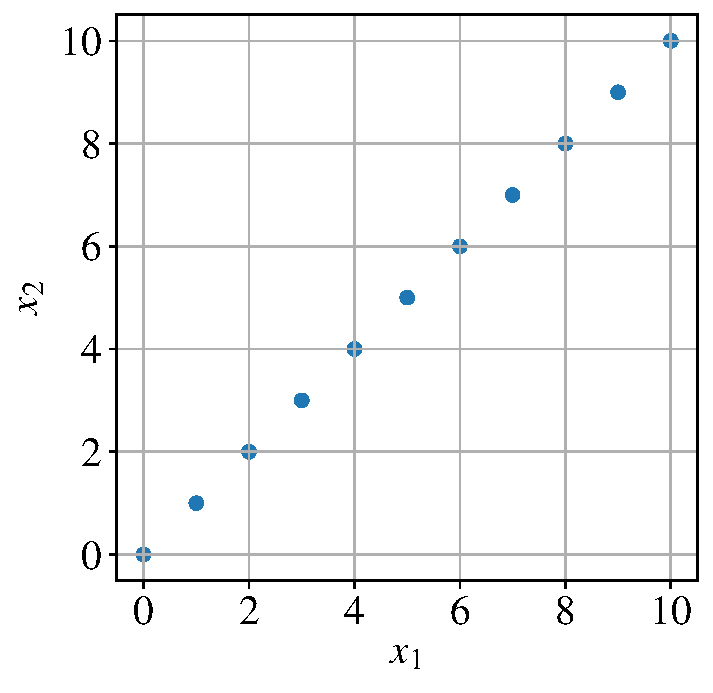
\includegraphics[width=0.4\textwidth]{figures/pca_2d}
  \caption{11 individus représentés par 2 variables $x_1$ et $x_2$.}
  \label{fig:pca_2d}
\end{figure}




\paragraph{Question 2.} Parmi les affirmations ci-dessous, lesquelles sont vraies ? On considère un jeu de données $X \in \RR^{n \times p}$ de $n$ individus en $p$ dimensions.
\begin{itemize}
\item[$\square$] La réduction de dimension relève de l'apprentissage supervisé.
\item[$\square$] La réduction de dimension relève de l'apprentissage non-supervisé.
\item[$\square$] La réduction de dimension facilite la visualisation des données.
\item[$\square$] L'analyse en composantes principales de $X$ permet de créer jusqu'à $n$ nouvelles dimensions. 
\item[$\square$] Les nouvelles variables créées par une analyse en composantes principales sont des combinaisons linéaires des $p$ variables.
\item[$\square$] L'analyse en composantes principales de $X$ s'obtient par une décomposition spectrale de $X$.
\item[$\square$] La sélection de variables consiste à conserver uniquement les variables dont la variance est la plus faible.
\end{itemize}

\section*{Solution}
{%
\noindent
\rotatebox[origin=c]{180}{%
\noindent
\begin{minipage}[t]{\linewidth}
\paragraph{Question 1.} La direction de plus grande variation des données est
la diagonale d'équation $x_1 = x_2$. Ainsi, la première composante principale
est le vecteur directeur de la diagonale, de norme 1, soit donc
$\left(\frac{\sqrt{2}}2, \frac{\sqrt{2}}2\right).$ \newline


\paragraph{Question 2.} 
\begin{itemize}
\item La réduction de dimension peut relever de l'apprentissage supervisé (par
  exemple, l'élimination des variables indépendantes de l'étiquette requièrent
  évidemment une étiquette) ou de l'apprentissage non-supervisé (par
  exemple, l'ACP). Elle est cependant souvent plutôt classée dans
  l'apprentissage non-supervisé car il s'agit d'analyse exploratoire des
  données et non pas d'analyse prédictive, ce qui peut prêter à confusion.
\item[\rlap{$\checkmark$}$\square$] La réduction de dimension facilite la visualisation des données.
\item[$\square$] L'analyse en composantes principales de $X$ permet de créer jusqu'à $n$ nouvelles dimensions. \\
FAUX, elle permet de créer jusqu'à $p$ nouvelles dimensions.
\item[\rlap{$\checkmark$}$\square$] Les nouvelles variables créées par une analyse en composantes principales sont des combinaisons linéaires des $p$ variables.
\item[$\square$] L'analyse en composantes principales de $X$ s'obtient par une décomposition spectrale de $X$.\\
FAUX, il s'agit de la décomposition spectrale de $X^\top X$.
\item[$\square$] La sélection de variables consiste à conserver uniquement les variables dont la variance est la plus faible. \\
FAUX, \textit{une des techniques} de sélection de variables consiste à \textit{éliminer} les variables dont la variance est la plus faible. \\
\end{itemize}
\end{minipage}%
}%



%%% Local Variables:
%%% mode: latex
%%% TeX-master: "../../sdd_2025_poly"
%%% End:






%%% Local Variables:
%%% mode: latex
%%% TeX-master: "../sdd_2025_poly"
%%% End:
